\chapter{Introduction}
\label{chapter:chapter01}
\section{Research Context}
As the world becomes increasingly globalised, the content produced in languages other than that of the mother tongue increases, especially that in the English language, which turns out to be the dominant worldwide. The need to learn this language dramatically increases as time progresses, and traditional teaching methods do not provide enough for the entire population that needs to learn it. It is thus necessary to create alternatives that are more accessible and optimal for students who are often occupied by a very active pace of life and have little flexibility in their schedule to practice among their acquaintances.\\

One alternative to help learn a new language consists of a system in which students who do not know each other are grouped according to their topics of interest. In this manner, students practice the use of language according to having conversations about these interests and a similar level of experience, allowing all participants to understand and take part.\\

This thesis aims to determine an optimal manner to group students into different virtual groups so that they can improve their use of language and not be frustrated either because of the unattainable difficulty or because the topics do not suit their liking. There are several aspects that can make one grouping better than another; for example, the level of language proficiency must be relatively compatible, that is, very advanced students cannot be put together with beginners, as the advanced student gets bored with the difficulties of the beginner, and the latter does not understand what the advanced say. Additionally, it is sought that the interests of the students are compatible, in order to generate conversations of interest to all. For example, while some students may have sports among their subjects of interest, some prefer football and others prefer swimming. Another criterion is the intervention style of each student, which can be more or less active and more or less shy. Thus, if many shy and passive students are in the same room, it will be difficult to have an agile dynamic that makes the session entertaining. For this reason, it is proposed to address the problem as one of multi-objective optimisation, where the topics of conversation and the level of the student experience are the objectives to optimise. To this end, a mono-objective solution that combines the above criteria in a weighted aggregate function will be implemented. Then a comparison will be made of the results obtained with different genetic algorithms based on the mono-objective solution and the multi-objective solution. It is believed that through the use of a multi-objective strategy, the student's experience will improve significantly compared to existing methods of teaching and practising foreign languages.\\

\section{Problem Definition}

The problem is defined as a variation of the Stable Roommate Problem (SRP), which is a variation of the Stable Marriage Problem (SMP)~\cite{Iwama_SMP_variants}. Only in this case, individuals do not know each other, so they have no real preference; nevertheless, the preference is predicted based on the similarity of the level of experience in the foreign language of the student and the interest that is shared with the rest of the group. The above is based on the fact that these two factors directly affect the student's preference to belong to the group.\\

In addition to this, group size and participation styles are also considered as restrictions for the benefit of the rest of the system, as a person may prefer to belong to a group that has more in common with him/her; however, his/her way of participating can alter the behaviour of the rest of the group. For example, an outgoing student who participates too much in a conversation can prevent the rest of the group from participating; conversely, a group in which no one participates needs an outgoing student to initiate the conversations.\\

In the same way, the size of the group is defined dynamically to obtain homogeneous participation among its members. It is defined dynamically since the absence or presence of some students can affect the performance of the group, although its size is not considered ideal.\\

This research aims to obtain the most stable solution possible concerning the predicted preferences of students within a reasonable time. Although there are many examples and variations of SRP in the literature, there is no characterisation that adapts directly to the problem defined considering the groups as variables. SRP is considered as a NP-complete problem, so it is relevant to find a solution in different by the use of heuristics and meta-heuristics. A comparison between single-objective algorithms and multi-objective is suggested to find a good enough solution for this problem.

\section{Objectives}

Compare single-objective and multi-objective strategies to find stable studying groups based on their interests and levels of experience, and consider the group size and their participation as constraints.\\

The specific objectives that this entails are described below:

\begin{enumerate}
    
    \item Define stability and near-stability for the problem.

    \item Build an artificial data-set to compare the potential approaches.

    \item Define the relevant attributes and parameters to formulate the single-objective and multi-objective functions.

    \item Implement mono-objective strategies to generate solutions to the problem, which will be the basis for comparing the multi-objective solutions that are made.

    \item Implement and test different multi-objective strategies and compare them with the results obtained with the mono-objective strategies.

    \item Review the results and make a report indicating if a better result was reached with a multi-objective strategy and what was the algorithm that had the best results.
\end{enumerate}

\section{Hypothesis}

Multi-Objective algorithms can outperform single-objective algorithms in finding near-stable studying groups based on their interests and level of experience, while considering the group size and participation as constraints.\\

This research tries to respond the following questions:

\begin{itemize}

\item How stable are the solutions found?

\item Which advantages multi-objective algorithms may have against single-objective algorithms and vice-versa?

\item Is optimisation even necessary? (Can a random solution be improved using optimisation techniques?)

\item How does single-objective solutions are, compared with multi-objective ones?

\item Can a single-objective algorithm have a solution that belongs to the Pareto front?

\item Which single-objective algorithm outperforms the other single-objective algorithms for this problem?

\item Which multi-objective algorithm outperforms the other multi-objective algorithms for this problem?

\item Which algorithm results to be the best overall?

\end{itemize}
\clearpage

\section{Contributions}

Below is shown a list of the main contributions of this research. They were established to achieve the objectives and answer the questions previously raised.

\begin{itemize}
    \item Introduces the problem of Stable Student Groups (SSGP), based mostly in SMP and SRP and other similar combinatorial problems.
    \item Makes a comparison of optimisation of different preference criteria against the stability of the resulting groups.
    \item Establishes a way to solve SSGP with unknown preferences, using a predicted preferences based on a preference criteria.
    \item Defines a set of objective functions to help predict the preference of the students of a given data-set.
    \item Builds a synthetic data-set based on distribution data, determined by the objective functions previously defined.
    \item Defines a set of operators to be used for SSGP, based on small but significant changes to the groups. 
    \item Presents different models for the solution of SSGP, and a way to compare them.
    \item Presents an extensive analysis of the solutions found making use of different ways to compare single-objective algorithms to multi-objective algorithms in a ways that are considered fair.
\end{itemize}

\section{Solution Model}

The solution for the established SSGP follows a structure for optimisation using evolutionary algorithms. First, the objective functions that represent the objective of the problem are defined. Then a synthetic database is generated using the distribution data for several sources. This data will be evaluated by the objective functions. After that, the operators for the evolutionary algorithms are defined and tested. \\

Finally, single-objective algorithms and multi-objective algorithms are compared within them and with each other. These comparisons follow closely the one based on the one developed by Ishibuchi et al.~\cite{Ishibuchi_single_vs_multiobjective}, who compared single-objective algorithms with multi-objective algorithms. A diagram of the solution model can be seen in Figure~\ref{fig:solution_model}.

\begin{figure}[H]
    \centering
    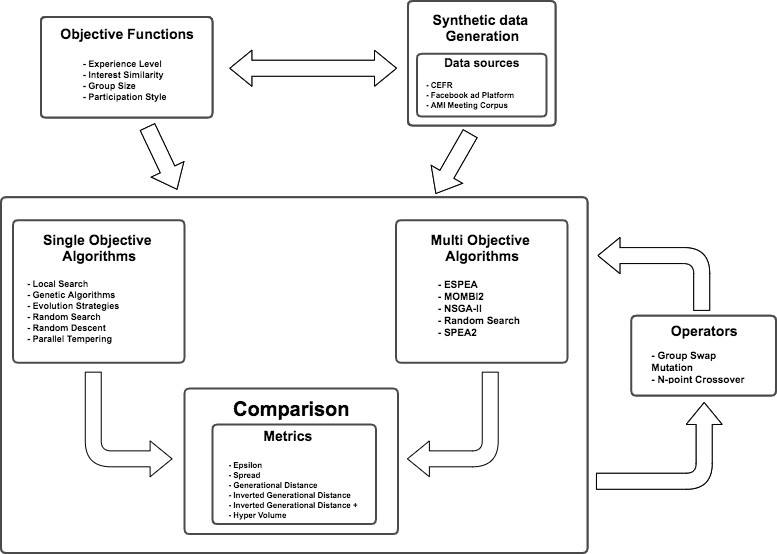
\includegraphics[width=\textwidth]{images/solution_model.png}
    \caption{Solution model proposed to compare the approaches to solve SSGP.}
    \label{fig:solution_model}
\end{figure}

\section{Document Structure}

Including this introduction, the thesis consists of 6 chapters. \\

Chapter~\ref{chapter:chapter02} provides a review of the literature. Includes basic definitions for the single-objective algorithms and multi-objective algorithms to be used. Additionally, it includes some background for performing a comparison between them, including the different metrics used. This chapter also discusses the preference criteria, which is later used to define the objective functions. Finally, it includes a brief introduction of the frameworks used to evaluate the different algorithms. \\

Chapter~\ref{chapter:chapter03} presents the design of the problem and the approach to solving it. It defines the objective functions to use and the operators for the different algorithms. \\

Chapter~\ref{chapter:chapter04} shows a set of preliminary experiments. Beginning to test the defined objective functions. Then, a brief methodology for the data-set creation is explained and later tested with a set of exploratory experiments. \\

Chapter~\ref{chapter:chapter05} contains the main experiments and a discussion of their results. The experiments are separated in the setup and three phases. The setup introduces the parameters to be used for the rest of the experimentation. The first phase contains the first set of experiments using the parameters defined in the setup. Second and Third phases are the result of the feedback obtained during the first phase. \\

Chapter~\ref{chapter:chapter06} explains the conclusions of the research and mentions the future work that can be derived.